Entropy fundamentally represents the minimal average number of bits required to encode information from a source. In the context of uniquely identifying objects within a set $U$, a related concept is the information content required, which serves as a fundamental measure of the space needed in compressed data representations. The primary goal of compressed data structures is to occupy space close to this theoretical lower bound, while simultaneously enabling efficient query operations. This balance between storage efficiency and query responsiveness is central to optimizing data compression techniques.

\noindent Numerous compression techniques exist, yet they often share certain fundamental steps. Figure \ref{fig:typical_processes} illustrates typical processes employed for data compression. These procedures depend on the nature of the data, and the specific arrangement or combination of the blocks shown may differ. Numerical manipulation, such as predictive coding and linear transformations, is commonly employed for waveform signals like images and audio. Logical manipulation involves transforming the data into a format more amenable to compression, including techniques such as run-length encoding, zero-trees, set-partitioning information representations, and dictionary methods. Subsequently, source modeling is used to estimate the data's statistical properties, which is crucial for effective entropy coding.

\begin{figure}[h]
    \centering
    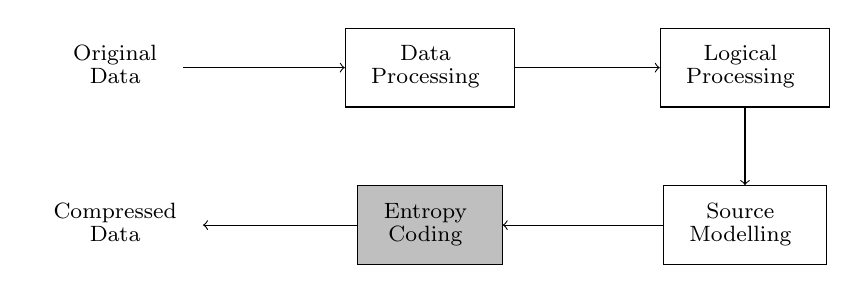
\begin{tikzpicture}
        \renewcommand{\arraystretch}{0.7} % Adjust line spacing in the tabular environment
        % Blocks
        \node (block1) at (0,0) {
            \begin{tabular}{c}
                \footnotesize Original \\
                \footnotesize Data
            \end{tabular}
        };
        \node[draw, minimum width=1cm, minimum height=1cm, align=center] (block2) at (4,0) {
            \begin{tabular}{c}
                \footnotesize Data \\
                \footnotesize Processing
            \end{tabular}
        };
        \node[draw, minimum width=1cm, minimum height=1cm, align=center] (block3) at (8,0) {
            \begin{tabular}{c}
                \footnotesize Logical \\
                \footnotesize Processing
            \end{tabular}
        };
        \node[draw, minimum width=1cm, minimum height=1cm, align=center] (block4) at (8,-2) {
            \begin{tabular}{c}
                \footnotesize Source \\
                \footnotesize Modelling
            \end{tabular}
        };
        \node[draw, minimum width=1cm, minimum height=1cm, align=center, fill=lightgray] (block5) at (4,-2) {
            \begin{tabular}{c}
                \footnotesize Entropy \\
                \footnotesize Coding
            \end{tabular}
        };
        \node (block6) at (0,-2) {
            \begin{tabular}{c}
                \footnotesize Compressed \\
                \footnotesize Data
            \end{tabular}
        };

        % Arrows
        \draw[->] (block1) -- (block2);
        \draw[->] (block2) -- (block3);
        \draw[->] (block3) -- (block4);
        \draw[->] (block4) -- (block5);
        \draw[->] (block5) -- (block6);

    \end{tikzpicture}
    \caption{Typical processes in data compression}\label{fig:typical_processes} % Consider adding citation if adapted, e.g., (Adapted from [Source])
\end{figure}

\noindent These initial numerical and logical processing stages typically aim to transform the data, exploiting specific properties like signal correlation or symbol repetition, to reduce specific forms of redundancy and produce a representation more amenable to statistical compression (e.g., yielding symbols with a more skewed frequency distribution or more predictable patterns). A common feature among most compression systems is the incorporation of \emph{entropy coding} as the final process, wherein the processed information is represented in a highly compact form. This stage can significantly impact the overall compression ratio, as it performs the final reduction in data size based on the modeled statistics. In this chapter, we examine the principles of entropy coding, exploring the fundamental concepts and methods that underpin this crucial stage of data compression.

\section{Worst-Case Entropy} \label{sec:worst_case_entropy}
When considering the task of assigning a unique identifier (\emph{code}, see \autoref{sec:source_and_codes}) to every element of a finite set $U$, a baseline measure of the required information content is the logarithm of the set size. If we constrain the codes to all have the same length $l$, then $l$ must be at least $\lceil \log_2 |U| \rceil$ bits to distinguish all elements. The theoretical minimum information content per element, expressed in bits, without the constraint of integer code lengths or specific coding schemes, is defined as the \emph{worst-case entropy} of $U$ \cite{ElementsofInformationTheory}
\begin{equation}
    H_{wc}(U) = \log_2 |U|
    \label{eq:worst_case_entropy_def}
\end{equation}
where $|U|$ denotes the number of elements in the set $U$. The term "worst-case" here refers to the scenario where no probability distribution over the elements is assumed (or equivalently, a uniform distribution is assumed), and we seek the theoretical limit for encoding based solely on the set size.

\begin{remark}
    If fixed-length binary codes are used, their length $l$ must be an integer. To assign a unique code to each of the $|U|$ elements, we require $2^l \ge |U|$. Taking the logarithm base 2 gives $l \ge \log_2 |U|$. Since $l$ must be an integer, the minimum required length is $l_{min} = \lceil \log_2 |U| \rceil \ge H_{wc}(U)$.
\end{remark}

\begin{example}
    Let $\mathcal{T}_n$ denote the set of all general ordinal trees \cite{benoit2005representing} with $n$ nodes. In this scenario, each node can have an arbitrary number of children, and their order is distinguished. With $n$ nodes, the number of possible ordinal trees is the $(n-1)$-th Catalan number, given by:
    \begin{equation*}
        |\mathcal{T}_n| = C_{n-1} = \frac{1}{n} \binom{2n - 2}{n - 1}
    \end{equation*}
    Using the known asymptotic approximation for Catalan numbers derived from Stirling's formula, for large $n$:
    \begin{equation*}
        |\mathcal{T}_n| = C_{n-1} \approx \frac{4^{n-1}}{\sqrt{\pi}(n-1)^{3/2}} = \frac{4^n}{4\sqrt{\pi}(n-1)^{3/2}} = \frac{4^n}{n^{3/2}} \Theta(1)
    \end{equation*}
    \begin{align*}
        H_{wc} (\mathcal{T}_n) & = \log_2 |\mathcal{T}_n|                              \\
                               & = \log_2 \left( \frac{4^n}{n^{3/2}} \Theta(1) \right) \\
                               & = 2n - \Theta(\log_2 n)
    \end{align*}
    Thus, we have determined the minimum number of bits required to uniquely identify (encode) a general ordinal tree with $n$ nodes based solely on their count.
\end{example}
